%%%%%%%%%%%%%%%%%%%%%%%%%%%%%%%%%%%%%%%%%%%%%%%%%%%%%%%%%%%%%%%%%%%%%%
% How to use writeLaTeX: 
%
% You edit the source code here on the left, and the preview on the
% right shows you the result within a few seconds.
%
% Bookmark this page and share the URL with your co-authors. They can
% edit at the same time!
%
% You can upload figures, bibliographies, custom classes and
% styles using the files menu.
%
%%%%%%%%%%%%%%%%%%%%%%%%%%%%%%%%%%%%%%%%%%%%%%%%%%%%%%%%%%%%%%%%%%%%%%

\documentclass[12pt]{article}

\usepackage{sbc-template}
\usepackage{graphicx,url}
\usepackage[brazil]{babel}   
\usepackage[utf8]{inputenc}  
% \usepackage{hyperref}
\def\UrlBreaks{\do\/\do-}
\sloppy

\title{Desenvolvendo uma Aplicação Web para o Gerenciamento de Reservas de Ambientes}

\author{Igor Cotrim Santos\inst{1}, Luis Paulo da Silva Carvalho\inst{1}}

\address{Instituto Federal da Bahia (IFBA)\\
  Av. Sérgio Vieira de Melo, 3150 - Zabelê\\  
  Vitória da Conquista, Bahia, Brasil\\ 
  \email{igorcotrim.dev@gmail.com, luiscarvalho@ifba.edu.br}
}


\begin{document} 

\maketitle

\begin{abstract}
\textbf{Context:} The management of room reservations represents a crucial challenge in several contexts, including educational activities, research and institutional initiatives. This article proposes a solution to address this issue. \textbf{Goal:} This work presents the design and implementation of Reserve+, a reservation management system. The Reserve+ architecture relies on a back-end, developed using Strapi and PostgreSQL, and a front-end that employs technologies such as React, Next.js, Zustand, Typescript and Tailwind. The goal is to offer a flexible solution capable of meeting the diverse demands of educational institutions. \textbf{Method:} The development of Reserve+ included the development of a web software and the practical validation through meetings with potential users. These interactions aimed to obtain feedback to optimize the system. \textbf{Results:} Reserve+ has been validated with users to meet the specific needs of reservations management in educational environments. The adopted architecture provides an answer to the challenges faced in this context. \textbf{Conclusions:} This project stands out for offering a solution for managing reservations, providing a response to the specific demands of educational institutions. The proposed architecture presents itself as a significant contribution to the management of environmental reserves.
\end{abstract}
     
\begin{resumo} 
\textbf{Contexto:} A gestão de reservas de ambientes representa um desafio crucial em diversos contextos, incluindo atividades educacionais, pesquisas e iniciativas institucionais. Este artigo propõe uma solução para abordar essa questão. \textbf{Objetivo:} O trabalho apresenta a concepção e implementação do Reserve+, um sistema de gerenciamento de reservas de ambientes. A arquitetura do Reserve+ é construída sobre um back-end, desenvolvido utilizando Strapi e PostgreSQL, e um front-end que emprega tecnologias como React, Next.js, Zustand, Typescript e Tailwind. O objetivo é oferecer uma solução flexível capaz de atender às diversas demandas de instituições de ensino. \textbf{Método:} O desenvolvimento do Reserve+ englobou o desenvolvimento de um software web e validação prática por meio de encontros com usuários em potencial. Essas interações visaram obter feedback para otimizar o sistema. \textbf{Resultados:} O Reserve+ foi validado com usuários para atender às necessidades específicas de gestão de reservas em ambientes educacionais e institucionais. A arquitetura adotada proporciona uma resposta para os desafios enfrentados nesse contexto. \textbf{Conclusões:} Este projeto destaca-se por oferecer uma solução para o gerenciamento de reservas, proporcionando uma resposta para as demandas específicas de instituições de ensino. A arquitetura proposta apresenta-se como uma contribuição significativa para a gestão de reservas de ambientes.
\end{resumo}


\section{Introdução}

Impulsionadas pela tecnologia da informação, as instituições de ensino enfrentam desafios contínuos na busca por eficiência administrativa e aprimoramento das atividades acadêmicas. Uma dessas tarefas é o gerenciamento de reservas de ambientes. De acordo com \cite{sistemas}, um sistema de gestão de reservas centraliza diversas funções em uma única ferramenta, permitindo o gerenciamento eficiente de informações sobre disponibilidade, preços e serviços oferecidos. Com um sistema de reservas eficiente, é possível reduzir erros e garantir a satisfação dos usuários, além de otimizar a gestão dos recursos da empresa. Nesse contexto, sistemas informatizados têm se destacado como uma resposta eficaz para otimizar esse processo crucial.

Segundo \cite{administracao}, um dos principais benefícios de um sistema de reservas é a possibilidade de automatizar tarefas repetitivas, permitindo que a equipe se concentre em atividades que agregam valor ao cliente e ao negócio. Além disso, esses sistemas oferecem maior flexibilidade e agilidade na gestão das reservas, permitindo que os usuários façam reservas em tempo real e a qualquer momento, por meio de plataformas online ou aplicativos móveis.

Essas soluções automatizadas revolucionam o gerenciamento de reservas, substituindo métodos manuais morosos por processos ágeis e eficientes. No Instituto Federal de Educação, Ciência e Tecnologia da Bahia (IFBA), essa necessidade ressoa de forma tão relevante quanto em qualquer outra instituição.

De acordo com \cite{arquitetura}, a arquitetura de \textit{software} é uma estrutura que define os componentes do sistema, suas interações e o comportamento geral do sistema. A arquitetura é um elemento-chave na construção de sistemas de \textit{software} e a proposição de uma arquitetura de \textit{software} dedicada ao gerenciamento de reservas de ambientes promete enriquecer a qualidade do ensino e da pesquisa. Isso será possibilitado ao permitir que os usuários efetuem reservas antecipadas dos ambientes desejados, além de proporcionar uma visão abrangente da disponibilidade dos recursos, minimizando conflitos de horários e obstáculos ligados à disponibilidade de materiais e equipamentos.

Mais do que simplificar o processo de reserva, a proposta de arquitetura aqui descrita visa reduzir o tempo investido pelos usuários nessa etapa, aprimorar a gestão temporal dos responsáveis pelos espaços e aprofundar a eficácia operacional. 

Para atingir tal objetivo foram realizados alguns passos cruciais: a (i) a captura precisa dos requisitos do sistema, (ii) a definição criteriosa de sua arquitetura, (iii) a criação de um repositório de código aberto no GitHub\footnote{https://github.com}, (iv) a construção da arquitetura e (v) a validação de um sistema baseado na arquitetura junto a um potencial usuário. 

 Vale salientar que foi realizada uma captura dos requisitos, aproveitando o IFBA, como exemplo emblemático de instituição de ensino que necessita automatizar a gestão de ambientes, e, considerando que foi definida uma arquitetura e criado um sistema de informação, este trabalho pode contribuir para a otimização da gestão de reservas de ambientes não só no IFBA, mas em outros ambientes educacionais.

\section{Trabalhos Relacionados} \label{sec:trabalhos}

Em \cite{costa}, Breno Maia criou o SIGALab, um sistema de informação gerencial acadêmico para reservas de laboratórios do IFES Colatina, desenvolvido para solucionar problemas enfrentados pelos coordenadores de turno na gestão das reservas. O sistema é apresentado em um trabalho de conclusão de curso que oferece soluções inovadoras para reduzir gastos desnecessários com impressão de papel e toner, além de facilitar o gerenciamento das reservas e contribuir para uma melhor organização e aproveitamento dos recursos dos laboratórios. No seu desenvolvimento foi utilizada a \textit{framework} de desenvolvimento ágil conhecida como Laravel\footnote{ https://laravel.com}. O SIGALab apresenta diversas funcionalidades que podem facilitar o gerenciamento das reservas. Algumas das principais funcionalidades são: (i) cadastro de reservas: permite que os usuários cadastrem suas reservas de salas e laboratórios de forma simples e rápida, sem a necessidade de impressão de papéis. (ii) vigência das reservas fixas: permite que os usuários cadastrem reservas fixas, que se repetem semanalmente, mensalmente ou em outros intervalos de tempo, facilitando o planejamento de aulas e atividades. (iii) quadro de horários fixos: apresenta um quadro de horários fixos para cada sala e laboratório, permitindo que os usuários visualizem a disponibilidade das salas e laboratórios em tempo real. (iv) controle de status das reservas: permite que os usuários controlem o status de suas reservas, podendo alterá-las ou cancelá-las a qualquer momento. 

Em \cite{tofolo} o sistema concebido por Edson Tofolo\footnote{O sistema não foi nomeado pelo seu autor} oferece a capacidade de agendar aulas práticas e gerenciar os estoques de um laboratório quanto de uma sala de apoio ao ensino. Além disso, a reserva de ambientes, que inclui o agendamento das aulas práticas, engloba também a reserva de materiais e equipamentos, sendo que as bases de dados correspondentes são distintas para cada departamento. Este sistema apresenta algumas funcionalidades essenciais, tal como o cadastro de itens, o controle de estoques e a possibilidade de empréstimo de materiais e equipamentos para a realização de projetos por professores e alunos. Sua implementação foi realizada utilizando a linguagem Java\footnote{https://www.java.com/pt-BR/} e diversos \textit{frameworks} e componentes voltados para aplicações web.

Embora os projetos SIGALab e o sistema concebido por Tofolo (2015) pareçam oferecer soluções promissoras para a gestão de laboratórios e salas acadêmicas, há uma preocupação notável que merece atenção. Ambos os textos mencionam o desenvolvimento desses sistemas, mas não fornecem informações detalhadas sobre a disponibilidade do código-fonte ou qualquer abordagem de código aberto para esses projetos. A transparência e a acessibilidade são fundamentais em iniciativas acadêmicas desse tipo, uma vez que a comunidade acadêmica e os desenvolvedores interessados podem contribuir, aprimorar e adaptar essas soluções para atender às suas próprias necessidades. A ausência de informações sobre o acesso ao código-fonte levanta questões sobre a sustentabilidade e a continuidade desses projetos no longo prazo, assim como a possibilidade de compartilhar conhecimento valioso com a comunidade. Portanto, é essencial que os desenvolvedores considerem a importância de tornar essas soluções mais acessíveis e transparentes, promovendo assim um ambiente acadêmico mais colaborativo e eficiente.

\section{Arquitetura e Tecnologias para um Sistema de Reservas} \label{sec:arqui_e_tech}


De acordo com \cite{arquitetura}, a arquitetura de um sistema é fundamental para garantir a qualidade e eficiência do \textit{software}. Uma arquitetura bem elaborada e executada oferece benefícios como modularidade, manutenibilidade, escalabilidade, segurança e performance. A divisão do sistema em módulos independentes facilita a manutenção e a evolução do código ao longo do tempo. Além disso, uma arquitetura escalável permite que o sistema cresça e suporte um aumento no número de usuários e recursos.

Segundo \cite{Loh} o sistema de reservas, adota uma abordagem abrangente ao integrar dois tipos de sistemas de informação. Por um lado, incorpora um Sistema de Gestão de Suprimentos para o controle efetivo dos bens materiais da organização, abrangendo a gestão da composição, aquisição e fluxo de materiais ao longo de toda a cadeia produtiva. Por outro lado, incorpora um sistema de workflow, possibilitando o planejamento e controle eficaz do fluxo de trabalho, promovendo assim uma gestão integrada e eficiente do processo como um todo.

Em \cite{souto} pode-se ver que, durante o desenvolvimento de sistemas modernos, a arquitetura frequentemente é dividida em duas partes distintas: o \textit{front-end} e o \textit{back-end}. O \textit{front-end} lida com a interface do usuário, a apresentação visual e a interação direta com os usuários. O \textit{back-end} gerencia a lógica de negócios, a manipulação de dados e a comunicação com bancos de dados e outros sistemas externos. As tecnologias escolhidas para o desenvolvimento do \textit{front-end} e do \textit{back-end} não são meramente uma questão de preferência, mas sim uma estratégia pensada para atender às demandas do sistema. No \textit{front-end} do sistema de reservas, a escolha do React\footnote{https://react.dev}, Next.js\footnote{https://nextjs.org}, Zustand\footnote{https://github.com/pmndrs/zustand}, TypeScript\footnote{https://www.typescriptlang.org} e Tailwind\footnote{https://tailwindui.com} foi baseada na necessidade de criar uma interface dinâmica, reativa e estilizada.

A adoção do Strapi\footnote{https://strapi.io} no \textit{back-end} oferece um CMS (\textit{Content Management System} ou, em português, Sistema de gerenciamento de conteúdo) flexível que se estende para a criação de APIs (\textit{Application Programming Interfaces} ou, em português, Interface de programação de aplicações) personalizadas, permitindo a gestão robusta das reservas e a implementação de autenticação e autorização de forma integrada. O PostgreSQL\footnote{https://www.postgresql.org} foi escolhido como o banco de dados, devido à sua confiabilidade e capacidade de gerenciar eficientemente os dados de reserva.

A escolha dessas tecnologias visou manter a coesão na arquitetura. Ou seja, cada tecnologia foi selecionada para se integrar com as outras, criando um sistema coeso e eficiente, capaz de cumprir as demandas de um sistema de reservas de ambientes. A arquitetura final, dividida entre \textit{front-end} e \textit{back-end},  associada com as tecnologias mencionadas nesta seção, pode ser visualizada na Figura \ref{fig:arqui_e_tech}.

\begin{figure}[ht]
\centering
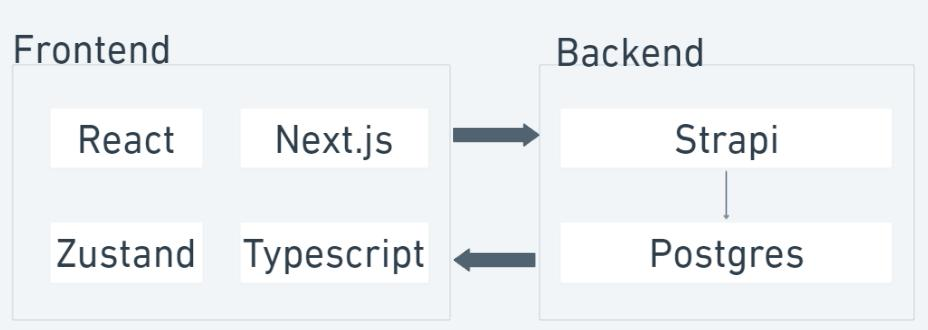
\includegraphics[width=0.8\textwidth]{arqui_e_tech.jpg}
\caption{Arquitetura Front-End x Back-End}
\label{fig:arqui_e_tech}
\end{figure}

As próximas seções descrevem as duas partes da arquitetura exibida na Figura \ref{fig:arqui_e_tech}.

\subsection{Front-end} \label{sec:front_end}

De acordo com \cite{kriger} o \textit{front-end} é uma parte do desenvolvimento de sistemas que se dedica a criar a parte visual e interativa de um site, aplicativo ou \textit{software}. É o que o usuário vê e usa quando acessa uma plataforma digital A arquitetura do \textit{front-end} é uma engrenagem essencial para a apresentação e interatividade, desempenhando um papel crucial no estabelecimento de uma experiência de usuário aprimorada.

A proposta para o \textit{front-end} da solução de gerenciamento de reservas de ambientes foi dividida nos módulos, evidenciados na Figura \ref{fig:front_end}:

(i) Módulo de autenticação: responsável pela autenticação e gerenciamento de usuários do sistema;
(ii) Módulo de visualização de reservas: responsável por exibir as reservas existentes em um calendário e permitir a interação do usuário com elas; (iii) Módulo de criação de reservas: responsável por permitir que os usuários criem novas reservas no sistema; (iv) Módulo de visualização de ambientes: responsável por exibir os ambientes existentes em uma tabela e permitir alguns filtros para achar a informação com mais facilidade; (v) Módulo de gerenciamento de solicitações: onde os responsáveis dos ambientes, vão conseguir aprovar ou reprovar as solicitações feitas para os ambientes.

A comunicação entre o \textit{front-end} e o \textit{back-end} foi alcançada por meio de APIs RESTful (\textit{Representational State Transfer} ou, em português, Transferência de Estado Representacional), promovendo a transferência de informações entre as duas partes.

\begin{figure}[ht]
\centering
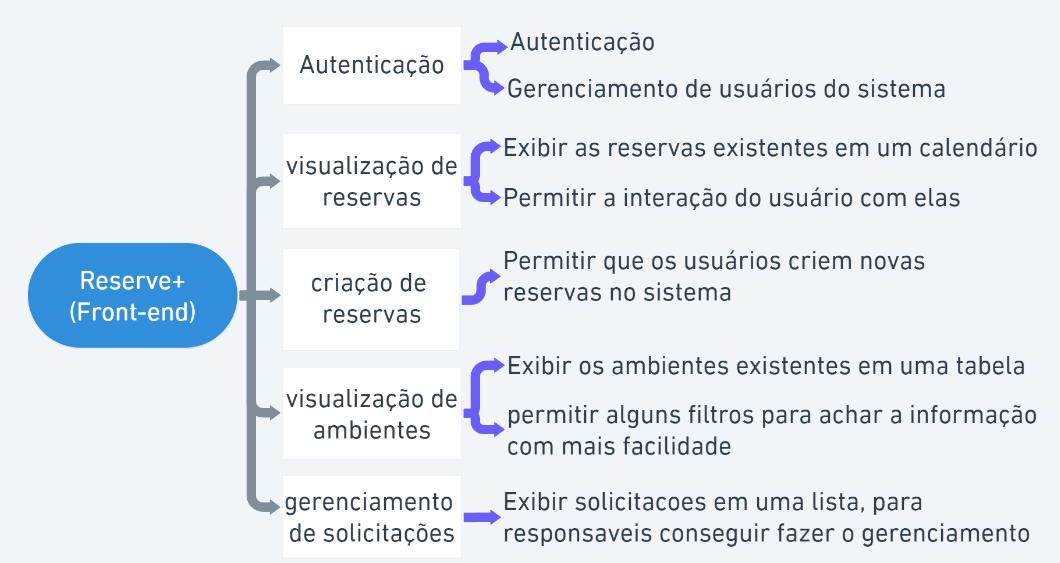
\includegraphics[width=1.0\textwidth]{front_end.jpg}
\caption{Modularização do Front-End}
\label{fig:front_end}
\end{figure}

\subsection{Back-end}\label{sec:back_end}

De acordo com \cite{clark} o \textit{back-end} é responsável por gerenciar o armazenamento de dados e prover as APIs para o \textit{front-end}. O \textit{back-end} é a parte de um aplicativo que os usuários não podem ver, mas está lá e funciona como a base de um grande produto de \textit{software}. O \textit{back-end} desenvolvido se encontra composto pelos seguintes módulos exibidos na Figura \ref{fig:back_end}:
(i) Módulo de autenticação e autorização: responsável por gerenciar a autenticação e autorização dos usuários no sistema, permitindo que apenas usuários autorizados possam realizar ações específicas; (ii) Módulo de gerenciamento de reservas: responsável por gerenciar as reservas de ambientes, permitindo a criação, atualização e exclusão de reservas; (iii) Módulo de gerenciamento de espaços: responsável por gerenciar as informações sobre os espaços disponíveis para reserva, incluindo informações sobre a capacidade, recursos disponíveis, disponibilidades e responsáveis; (iv) Módulo de gerenciamento de usuários: responsável por gerenciar as informações sobre os usuário, incluindo informações sobre a tipo de usuário, código e identificação eletrónica; (v) Módulo de gerenciamento de semestres: responsável por gerenciar as informações sobre os semestres, incluindo informações sobre qual é o semestre, início, fim e se é o semestre atual.

Esses módulos trabalham em conjunto para fornecer a funcionalidade geral do sistema de reservas, gerenciando a lógica de negócios e o armazenamento de dados necessários para o seu funcionamento.

\begin{figure}[ht]
\centering
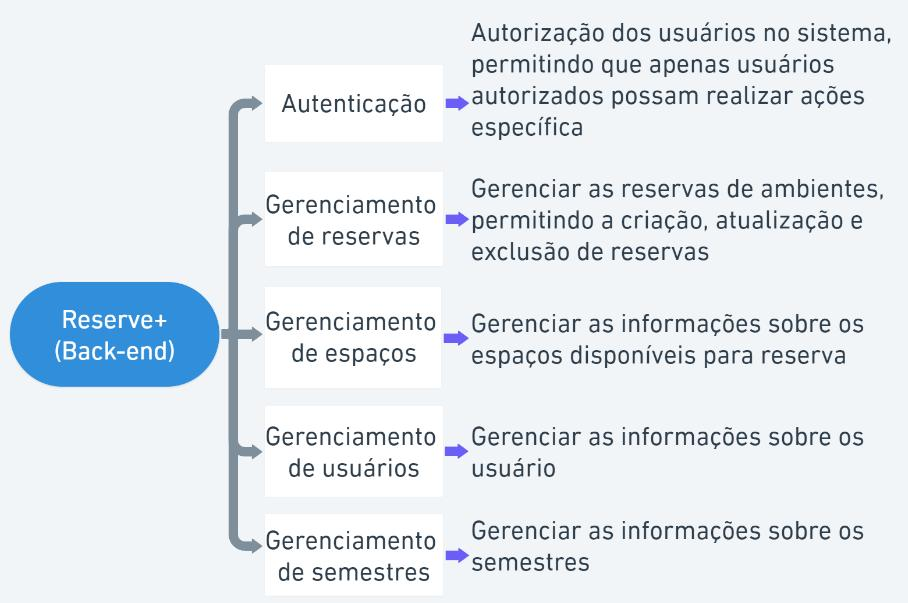
\includegraphics[width=1.0\textwidth]{back_end.jpg}
\caption{Modularização do Back-End}
\label{fig:back_end}
\end{figure}

\subsection{Conteinerização} \label{sec:conteinerizacao}

No desenvolvimento da arquitetura de \textit{software} para o gerenciamento de reservas de ambientes, adotamos uma abordagem orientada a contêineres. A conteinerização é uma prática amplamente reconhecida na indústria de TI que envolve o empacotamento de uma aplicação e suas dependências em um ambiente isolado conhecido como contêiner. Exploramos o uso de conteinerização, com destaque para a tecnologia Docker\footnote{https://www.docker.com}.

Segundo \cite{docker} a utilização de contêineres apresenta diversas vantagens para o desenvolvimento e a implantação de sistemas: (i) isolamento: os contêineres fornecem isolamento de recursos, garantindo que cada aplicativo em execução não afete o desempenho ou a estabilidade de outros aplicativos no mesmo \textit{host}. Isso evita conflitos entre dependências e facilita a implantação de aplicativos independentes,  (ii) portabilidade: os contêineres encapsulam o aplicativo e suas dependências, tornando-o altamente portátil. Um contêiner pode ser executado em qualquer ambiente que suporte a tecnologia de conteinerização, independentemente das diferenças de infraestrutura, (iii) eficiência: os contêineres compartilham o mesmo kernel do sistema operacional, o que os torna mais eficientes em termos de recursos em comparação com máquinas virtuais tradicionais. Isso resulta em um melhor aproveitamento dos recursos do servidor, (iv) escalabilidade: os contêineres são escaláveis, o que significa que é possível criar e destruir contêineres conforme a demanda. Isso facilita a escalabilidade horizontal de aplicativos, garantindo que eles possam lidar com um grande volume de tráfego quando necessário, (v) reprodutibilidade: a definição do ambiente de um contêiner é armazenada em um arquivo chamado Dockerfile, o que permite a reprodutibilidade do ambiente de desenvolvimento em qualquer lugar. Isso é fundamental para garantir que o aplicativo funcione de maneira consistente em diferentes estágios de desenvolvimento e implantação.

De acordo com \cite{docker} o Docker é uma tecnologia líder no campo da conteinerização. Ele oferece uma plataforma aberta para desenvolvimento, envio e execução de aplicativos em contêineres. Com o Docker, é possível criar, implantar e gerenciar contêineres de forma consistente em diversos ambientes, desde o desenvolvimento até a produção. Isso elimina as preocupações com diferenças de configuração entre ambientes, garantindo que o aplicativo funcione de maneira confiável em todas as fases do ciclo de vida.

\section{Desenvolvimento} \label{sec:desenvolvimento}

Considerando as decisões arquitetônicas descritas na Seção 3 e as tecnologias escolhidas, esta seção fornece mais detalhes sobre o processo de desenvolvimento do sistema chamado Reserve+.

O desenvolvimento do sistema é representado no fluxograma apresentado na Figura \ref{fig:processos_desenvolvimento_do_artigo}. Iniciou-se com a captura dos requisitos, um processo fundamental que abrange a identificação precisa das necessidades inerentes a esse tipo de solução. Nesse contexto, optamos por utilizar o caso do IFBA como uma sólida fonte de requisitos, buscando assegurar uma compreensão abrangente e alinhada com as expectativas. Em seguida, adentramos à etapa crucial da definição da arquitetura, a qual foi precedida por pesquisas em trabalhos relacionados. A organização do projeto foi otimizada com a criação de um repositório no GitHub, proporcionando uma gestão eficaz do código-fonte. A implementação da arquitetura seguiu-se como uma etapa subsequente, transformando a teoria em prática e materializando o sistema. Para assegurar a eficácia do resultado, realizamos uma validação com um usuário potencial, garantindo assim que as funcionalidades às necessidades identificadas.

\begin{figure}[ht]
\centering
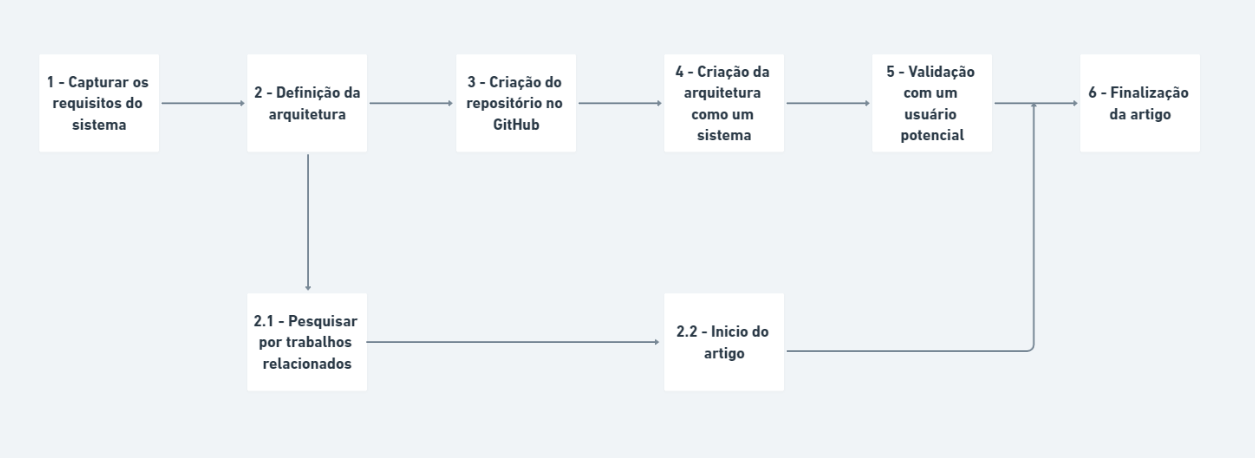
\includegraphics[width=1.0\textwidth]{processos_desenvolvimento_do_artigo.png}
\caption{Fluxograma do projeto}
\label{fig:processos_desenvolvimento_do_artigo}
\end{figure}

Para o desenvolvimento do \textit{front-end}, utilizamos as tecnologias React, Next.js, Zustand, Tailwind e TypeScript, como apresentado na Seção 3.1. 

O Next.js, \textit{framework} baseado na biblioteca React, foi utilizado para facilitar a renderização do lado do servidor, melhorar o desempenho e otimizar a experiência do usuário. O zustand foi utilizado para gerenciamento de estado e permitir que a aplicação seja escalável e fácil de ser mantida. A utilização do Tailwind facilita o desenvolvimento do \textit{front-end}, pois permite a criação de estilos de forma ágil, sem a necessidade de escrever CSS customizado o que deixa a responsividade mais fácil de ser implementada. Por fim, o TypeScript foi utilizado para adicionar tipagem estática\footnote{É um recurso que permite especificar tipos de dados para variáveis, parâmetros de função e valores retornados, garantindo que o código seja mais seguro e menos propenso a erros durante a compilação, ao mesmo tempo em que fornece ferramentas para ajudar os desenvolvedores a entender e manter o código com mais facilidade} à aplicação, garantindo maior confiabilidade e robustez ao código.

Para implementar o \textit{back-end}, utilizamos o CMS, Strapi, que é construído sobre a plataforma Node.js e permite a criação rápida de APIs personalizadas. O Strapi fornece um painel de administração para gerenciamento de conteúdo e autenticação de usuários, além de permitir a configuração de \textit{endpoints} de API personalizados para atender às necessidades da aplicação. Para o banco de dados, foi utilizado o PostgreSQL. 

O PostgreSQL é compatível com várias linguagens de programação e fornece recursos avançados de segurança e controle de acesso. Utilizamos a linguagem de programação JavaScript para escrever as rotas personalizadas do Strapi e as funções de acesso ao banco de dados.

A Figura \ref{fig:exemplo_solicitacao} mostra a solicitação de reserva vinda do \textit{front-end}, passando pelo Strapi e logo depois sendo gravada no banco de dados.

\begin{figure}[ht]
\centering
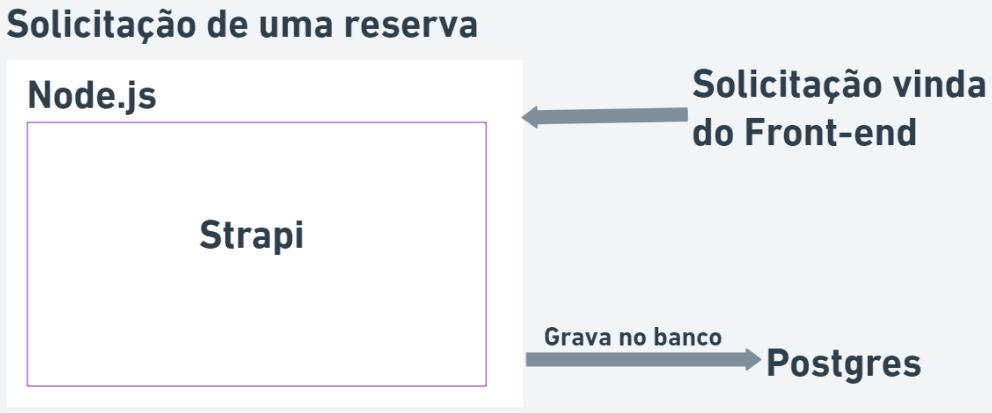
\includegraphics[width=0.8\textwidth]{exemplo_solicitacao.jpg}
\caption{Exemplo de uma Solicitação de Reserva}
\label{fig:exemplo_solicitacao}
\end{figure}

\subsection{O Front-end Resultante} \label{sec:front_end_resultante}

Esta seção é dedicada a demonstrar o resultado da implementação do \textit{front-end} da solução. É possível visualizar algumas das telas do Reserve+, sendo a Figura \ref{fig:front_end_resultante} a tela inicial. 

A tela principal representa o ponto de entrada do usuário ao acessar o sistema. Nela, ele terá uma visão geral das funcionalidades oferecidas por cada seção, acompanhada de informações descritivas e imagens ilustrativas. O objetivo é deixar o \textit{front-end} o mais intuitivo possível através da exibição de informações sobre o seu uso.

\begin{figure}[ht]
\centering
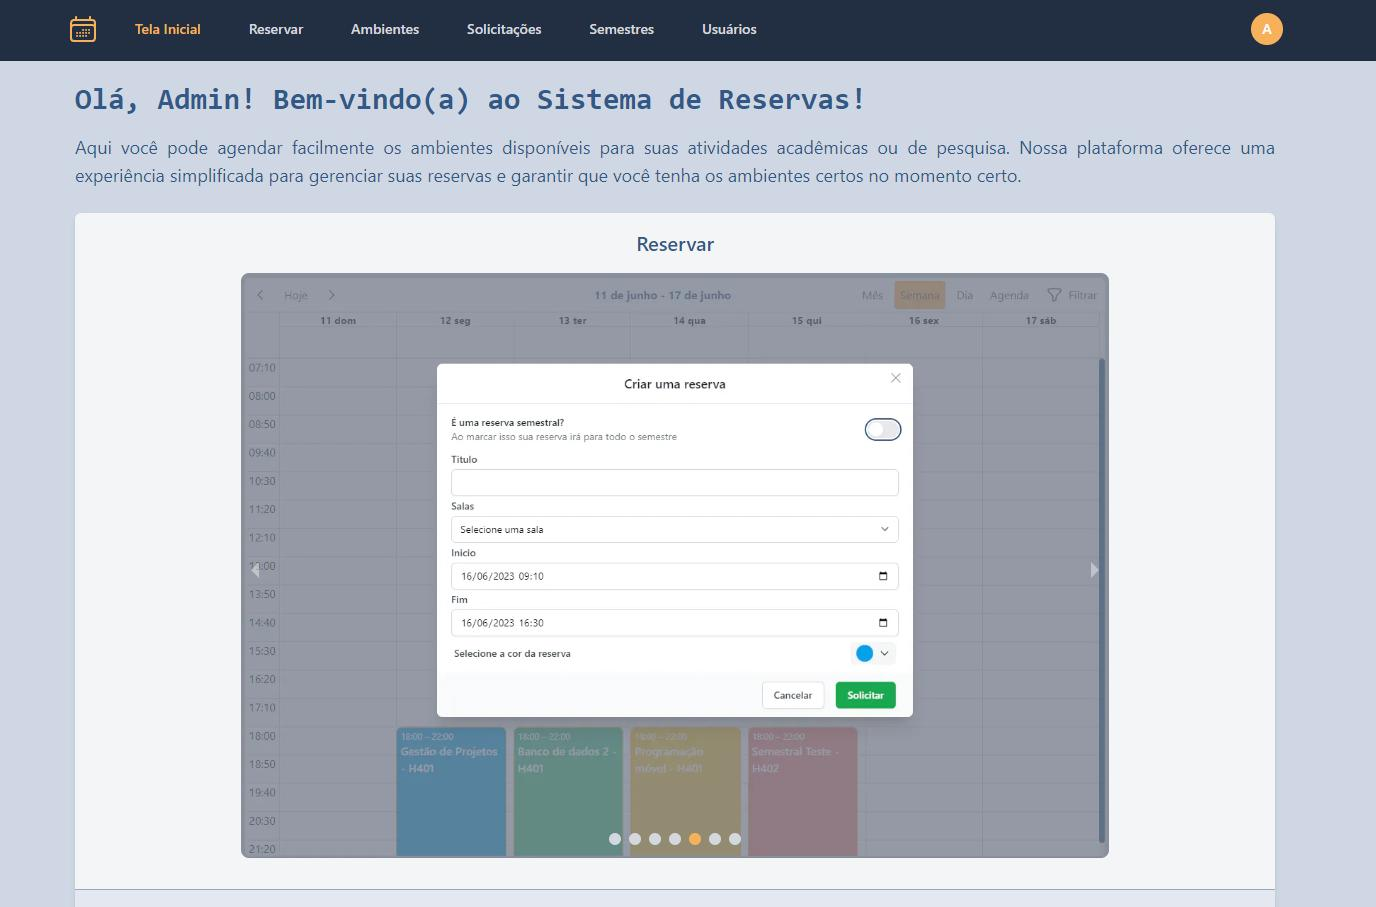
\includegraphics[width=1.0\textwidth]{front_end_resultante.jpg}
\caption{O Front-end Resultante}
\label{fig:front_end_resultante}
\end{figure}

A Figura \ref{fig:tela_reservar} retrata a tela de reserva, correspondente à visualização do calendário. Nesta tela, o usuário é capaz tanto de visualizar quanto criar reservas para diversos espaços disponíveis. A tela permite filtrar as reservas de acordo com o tipo (sejam elas semestrais ou pontuais) e ambiente escolhido. Além disso, oferece a flexibilidade de alternar entre diferentes modos de visualização, abrangendo opções como mês, semana, dia ou até uma visualização de agenda. Nesta última, o usuário vê em forma de lista, todas as reservas do dia atual até um  mês no futuro.

\begin{figure}[ht]
\centering
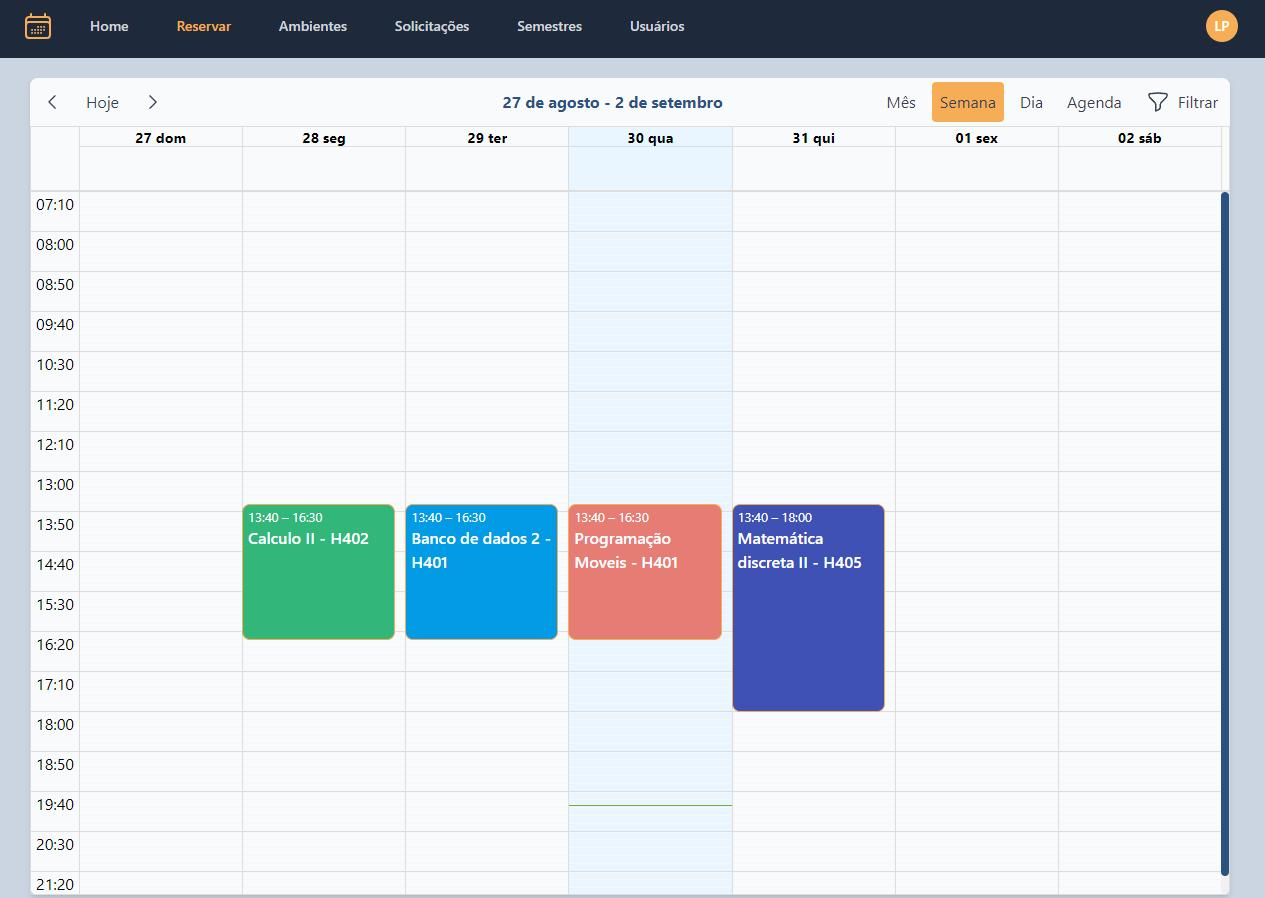
\includegraphics[width=1.0\textwidth]{tela_reservar.jpg}
\caption{Tela Reservar do Reserve+}
\label{fig:tela_reservar}
\end{figure}

A Figura \ref{fig:tela_ambientes} ilustra a tela dedicada ao cadastro de ambientes. Nesta tela, os usuários têm a capacidade de acessar informações detalhadas sobre os diferentes espaços disponíveis, além de dispor de opções de filtragem com base no tipo de ambiente e em sua disponibilidade.

\begin{figure}[ht]
\centering
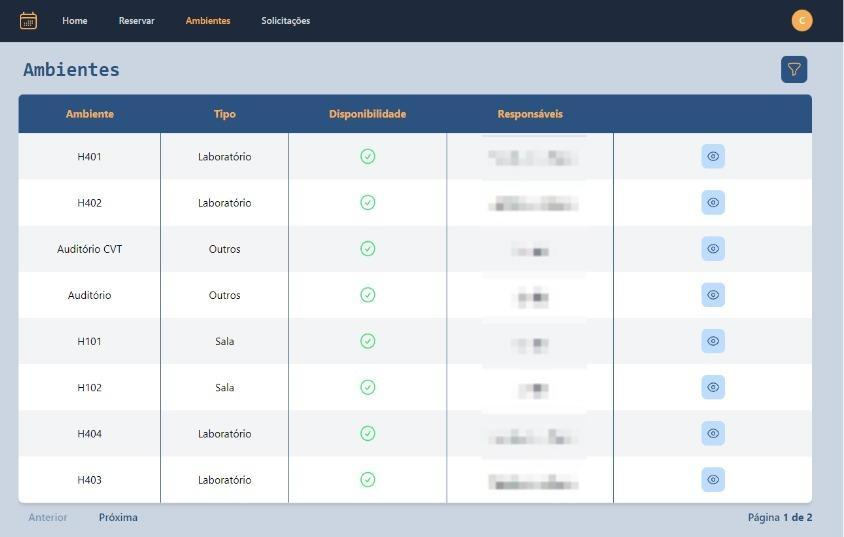
\includegraphics[width=1.0\textwidth]{tela_ambientes.jpg}
\caption{Tela Ambientes do Reserve+}
\label{fig:tela_ambientes}
\end{figure}

Para os usuários com privilégios administrativos, uma opção adicional é o botão "Criar Ambiente". Essa funcionalidade permite a esses administradores criar novos espaços, além de efetuar operações como a exclusão e atualização de ambientes já existentes. Isso confere ao sistema um controle flexível e abrangente sobre a gestão dos espaços físicos.

A Figura \ref{fig:tela_solicitacoes} apresenta a interface destinada às solicitações de reservas de ambientes. Essa tela permite que usuários, no papel de responsáveis pelos ambientes, aceitem ou reprovem as solicitações de reserva que foram submetidas.

\begin{figure}[ht]
\centering
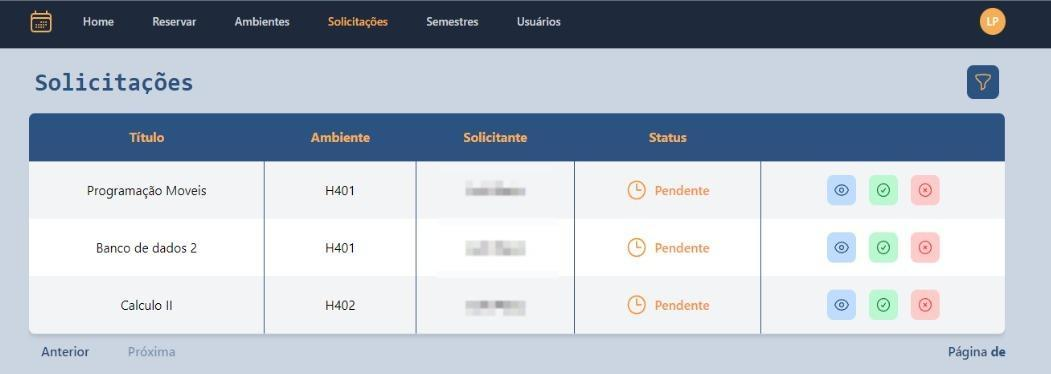
\includegraphics[width=1.0\textwidth]{tela_solicitacoes.jpg}
\caption{Tela Solicitações do Reserve+}
\label{fig:tela_solicitacoes}
\end{figure}

\subsection{O Back-end Resultante} \label{sec:back_end_resultante}

A adoção do Strapi como a base do \textit{back-end} do Reserve+ foi uma decisão estratégica, impulsionada pela facilidade de uso, capacidade de criação de APIs personalizadas e robustos recursos de autenticação e autorização.

Com o Strapi, a configuração e o gerenciamento do \textit{back-end} ocorreram de maneira intuitiva, permitindo a adaptação precisa às necessidades do sistema. Na Figura \ref{fig:strapi}, é possível observar o painel administrativo do Strapi, onde os administradores podem inserir e gerenciar dados (por meio do item do menu denominado "\textit{Content Manager}"), enquanto os desenvolvedores têm a capacidade de criar tabelas personalizadas (utilizando o item do menu chamado "\textit{Content-Type Builder}"), além de acessar uma variedade de configurações avançadas. Essa escolha estratégica garante uma base sólida e altamente flexível para o sistema, contribuindo significativamente para sua eficácia e segurança.

\begin{figure}[ht]
\centering
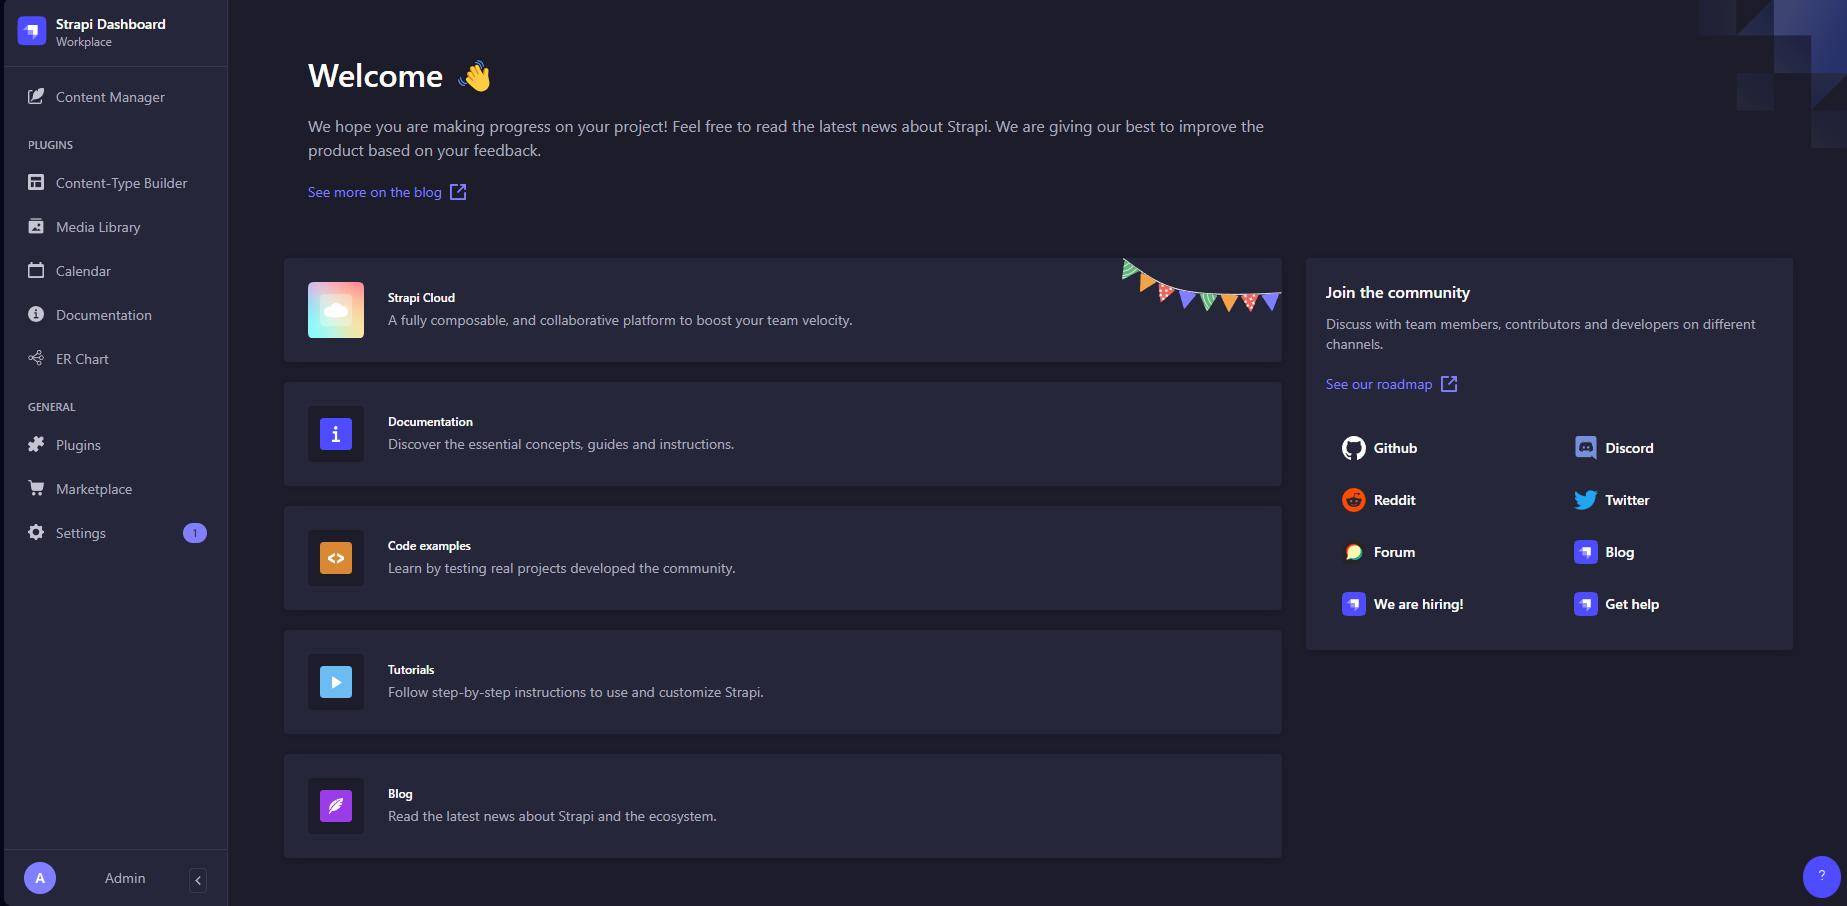
\includegraphics[width=1.0\textwidth]{strapi.jpg}
\caption{Tela inicial do painel administrativo do Strapi do Reserve+}
\label{fig:strapi}
\end{figure}

Na Figura \ref{fig:tabelas}, pode-se ver o diagrama de tabelas do banco de dados que inclui as seguintes entidades: (i) \textit{ambience}: mantém informações sobre os ambientes disponíveis para reserva, incluindo capacidade, recursos e disponibilidade. (ii) \textit{user}: armazena informações sobre os usuários, incluindo nome, endereço de e-mail e senhas criptografadas para fins de autenticação. (iii) \textit{admin-user}: armazena informações sobre os usuários do painel administrativo do Strapi, incluindo nome, endereço de e-mail e senhas criptografadas para fins de autenticação. (iv) \textit{reservation}: registra detalhes sobre cada reserva, como data inicial e data final, se é uma reserva semestral,  ambiente, solicitante e status da reserva. (v) \textit{semester}: armazena dados relacionados aos semestres acadêmicos, como se é semestre atual e datas de início e término.

\begin{figure}[ht]
\centering
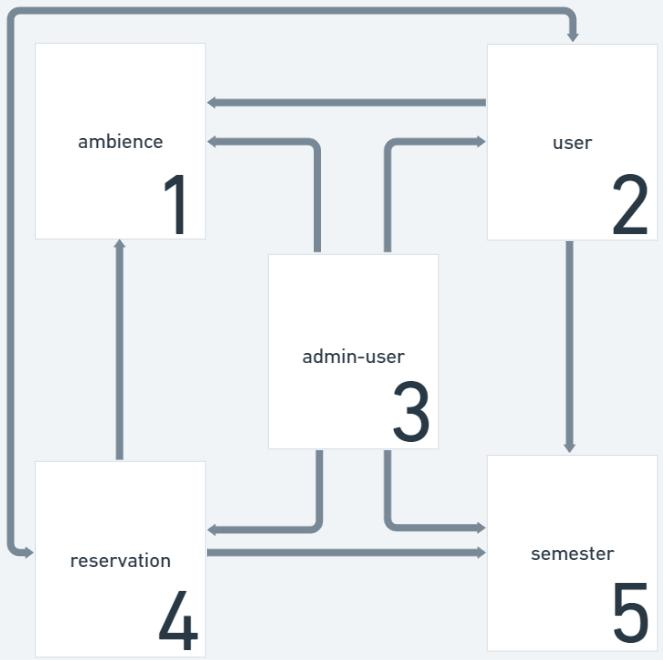
\includegraphics[width=0.7\textwidth]{tabelas.jpg}
\caption{Diagrama de Tabelas}
\label{fig:tabelas}
\end{figure}

\subsection{Infraestrutura de contêineres} \label{sec:conteineres}

A infraestrutura de contêineres oferece flexibilidade e escalabilidade para o Reserve+. Ambos o \textit{front-end} e o \textit{back-end} são hospedados em contêineres, o que permite uma gestão eficiente dos recursos e uma implantação simplificada. Na tabela \ref{tab:containeres}, mostra 3 contêineres no Docker, para o sistema. Sendo o \textit{client}, o contêiner que abriga o \textit{front-end} da aplicação, que inclui a interface do usuário e as funcionalidades visíveis para os usuários. É aqui que ocorre a interação direta com os solicitantes de reservas e os responsáveis pelos ambientes. O \textit{server}, o contêiner que abriga o \textit{back-end} do sistema que gerencia o armazenamento de dados, a autenticação e a comunicação com o \textit{front-end}. Este contêiner abriga o Strapi, garantindo que todos os processos de \textit{back-end} funcionem de maneira eficaz. E por último, o \textit{serverDB}, o contêiner que abriga o banco de dados, o PostgreSQL, utilizado para armazenar dados críticos, como informações de reservas, usuários e ambientes.

\begin{table}[ht]
\centering
\caption{Contêineres do Reserve+}
\label{tab:containeres}
\begin{tabular}{ |c|c| } 
 \hline
 \textbf{Reserve+} & \textbf{Contêineres} \\ 
 \hline
 front-end & Client \\ 
 \hline
 back-end & Server \\ 
 \hline
 banco de dados & ServerDB \\ 
 \hline
\end{tabular}
\end{table}

\section{Validação do sistema} \label{sec:validacao}

Durante o processo de desenvolvimento do sistema, optamos por adotar uma abordagem ágil, visando aprimorar a comunicação e a colaboração entre o desenvolvedor (discente autor deste trabalho) e um usuário potencial, docente do curso de Bacharelado em Sistemas de Informação do IFBA, campus Vitória da Conquista, que lida constantemente com as reservas de ambientes.

Realizamos encontros periódicos com o usuário, buscando obter \textit{feedback} direto para o aperfeiçoamento contínuo da solução. Essa interação permitiu identificar as necessidades e expectativas do usuário, possibilitando ajustes e melhorias ao longo do desenvolvimento. (i) Versão 1: Foi desenvolvido somente o \textit{front-end}. Durante essa análise, foram identificados diversos aspectos visuais que requerem atenção. Por exemplo, foi observada a carência de um recurso de filtragem nas telas que apresentam listagens. Além disso, destacou-se a importância de incorporar um mecanismo para a fácil remoção dos filtros aplicados. Outro ponto de destaque foi a necessidade de permitir a personalização da cor das reservas exibidas no calendário. Foi sugerido também que a visualização padrão do calendário fosse semanal, e que fosse incluída uma opção para visualizar todas as reservas em um intervalo de tempo; (ii) Versão 2: Já integrada com o \textit{back-end}. Durante a avaliação, foram identificados outros aspectos a serem aprimorados. Por exemplo, foi observada a necessidade de incluir um campo de motivo ao reprovar uma solicitação de reserva. Além disso, foi sugerido renomear o item de menu "Calendário" para "Reservar" (para evidenciar melhor qual é a ação resultante ao se usar a tela) e criar uma tela inicial que ofereça orientações ao usuário sobre o funcionamento do sistema. Outro requisito enfatizado foi a implementação de um perfil de usuário administrador no \textit{front-end}, permitindo a realização de tarefas como a inserção de dados referentes a semestres, usuários e ambientes. Além disso, foi destacada a importância de incorporar um recurso de filtro no calendário, com a observação de que esse filtro deveria estar inicialmente aberto por padrão e a limitação de horários no calendário; (iii) Versão 3: Incorporando todas as melhorias discutidas na reunião anterior. O feedback do usuário foi positivo, e surgiu a sugestão de hospedar o projeto em um servidor no IFBA, permitindo que outros usuários também possam utilizá-lo e oferecer uma validação mais abrangente.

Após o período de realização dos encontros, o sistema foi instalado em duas máquinas, uma remota, online (link na Seção 6, Tabela 2), e outra local, nas dependências do IFBA. O objetivo do uso de uma máquina local seria permitir o uso interno do Reserve+ para gerenciar os ambientes do IFBA. Contudo, até a presente data, a infraestrutura local ainda não está disponível.

Mesmo após a instalação, o processo de desenvolvimento e melhoria do \textit{software} continuou. Entre as melhorias, destacam-se: (i) inclusão do número de máquinas na listagem de ambientes, permitindo que os usuários visualizem de forma imediata a quantidade de máquinas disponíveis nos laboratórios, sem a necessidade de acessar informações detalhadas; (ii) implementação de um filtro por número de máquinas na listagem de ambientes, facilitando a busca e seleção de ambientes de acordo com a quantidade de máquinas desejada; (iii) adequação na ordenação dos ambientes, categorizando-os corretamente como laboratórios, salas e outros, para proporcionar uma organização mais intuitiva; (iv) adição de um campo na criação de ambientes, permitindo a especificação dos \textit{softwares} instalados nos computadores dos laboratórios. Isso proporcionará aos docentes informações sobre os recursos disponíveis ao reservar um laboratório; (v) aprimoramento do formulário de criação de reserva, incluindo informações sobre o ambiente, tais como: o nome da sala, a capacidade de pessoas e o número de máquinas disponíveis, no caso de laboratórios.

\section{Resultado} \label{sec:resultado_final}

Nesta seção, se concentram informações sobre as principais contribuições deste trabalho. 

Acessando o link do repositório no GitHub (https://github.com/reservas-de-ambientes/reserveplus), é possível explorar o código-fonte do sistema, visualizar o sistema implementado e ter uma compreensão mais aprofundada de como as tecnologias e estratégias discutidas neste artigo foram aplicadas na prática.

Ao acessar o link do vídeo no YouTube (https://www.youtube.com/watch?v=BiqJOwknfeU), é possível assistir a um vídeo abordando o uso do Reserve+. Durante este vídeo, é explorada sua interface, além de ser examinado como ele utiliza contêineres Docker e visualizar as funcionalidades do painel administrativo, que é gerenciado pelo Strapi.

Com o objetivo de realizar testes, optou-se por hospedar o \textit{front-end} na plataforma Vercel\footnote{https://vercel.com}, enquanto o \textit{back-end} e o banco de dados foram alocados no Render\footnote{https://render.com}. Isso possibilitou a implantação na nuvem de maneira econômica. No entanto, devido à configuração específica, não foi possível aproveitar a infraestrutura de contêineres Docker, o que resultou na impossibilidade de testar essa funcionalidade na nuvem. Ao acessar o link do Projeto Reserve+ (https://reserveplus.vercel.app), é possível explorar as funcionalidades disponíveis na plataforma para cada tipo de usuário. A Figura \ref{fig:funcionalidades} ilustra como as funcionalidades se encontram divididas por cada um.

\begin{figure}[ht]
\centering
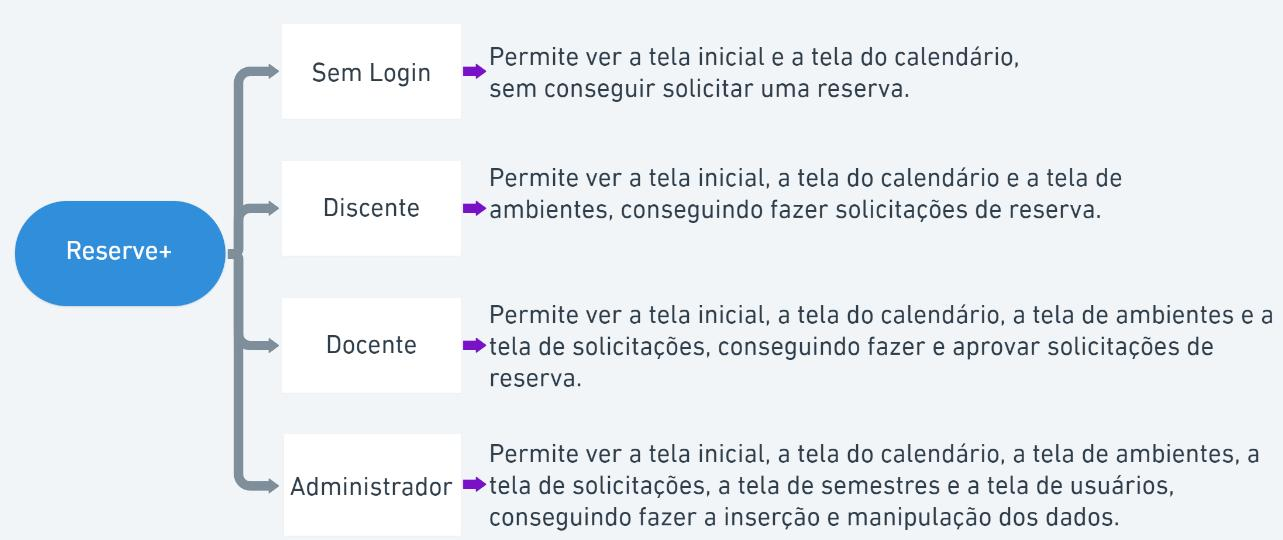
\includegraphics[width=1.0\textwidth]{funcionalidades_por_usuario.jpg}
\caption{Funcionalidades por Usuário}
\label{fig:funcionalidades}
\end{figure}

Para acessar as diferentes contas, podem ser utilizadas as seguintes credenciais: (i) conta de administrador: login, \textit{admin@gmail.com}, senha, \textit{admin12345}, (ii) conta de discente: login, \textit{discente@gmail.com}, senha, \textit{discente12345}, (iii) conta de docente: login, \textit{docente@gmail.com}, senha, \textit{docente12345}. 

Ao acessar o link do Painel Administrativo do Reserve+ (https://strapi-oz03.onrender.com/admin), é possível visualizar as entidades do sistema e realizar lançamentos diretamente, com os privilégios de super administrador. Para acessar, as seguintes credenciais devem ser utilizadas: (i) login, \textit{admin@admin.com}, senha, \textit{Admin12345}.

A Tabela \ref{tab:contribuicoes} fornece um QR Code para visualizar os detalhes sobre cada link de contribuição mencionada. 

\begin{table}[ht]
\centering
\caption{Detalhes sobre cada Contribuição}
\label{tab:contribuicoes}
\begin{tabular}{ |c|c| } 
 \hline
 \textbf{Link} & \textbf{QR Code} \\ 
 \hline
 Github (https://abrir.link/nsXTM) & 
 \begin{minipage}{.3\textwidth}
    \centering
    
\includegraphics[width=0.8\textwidth]{github.jpg}
 \end{minipage}
 \\ 
 \hline
 Youtube (https://abrir.link/hNIUB) & 
 \begin{minipage}{.3\textwidth}
    \centering
    
\includegraphics[width=0.8\textwidth]{youtube.jpg}
 \end{minipage}
 \\ 
 \hline
 Reserve+ (https://abrir.link/xQJhv) & 
  \begin{minipage}{.3\textwidth}
    \centering
    
\includegraphics[width=0.8\textwidth]{reserve+.jpg}
 \end{minipage}
 \\
 \hline
 Painel Administrativo (https://abrir.link/jfX2I) & 
  \begin{minipage}{.3\textwidth}
    \centering
    
\includegraphics[width=0.8\textwidth]{administrativo.jpg}
 \end{minipage}
 \\ 
 \hline
\end{tabular}
\end{table}

\section{Conclusões e Trabalhos Futuros}

Este artigo delineou uma arquitetura de \textit{software} planejada para o gerenciamento de reservas de ambientes. Através da escolha e integração de tecnologias, o \textit{front-end} e o \textit{back-end} foram articulados visando proporcionar  o uso do sistema de informação resultante por instituições de ensino.

Além da abordagem arquitetural e de uso de tecnologias atuais, um processo de desenvolvimento ágil foi utilizado para permitir a interação frequente com um usuário potencial do sistema. Isto permitiu ajustes oportunos e alinhamento às necessidades reais, traduzindo-se em um sistema potencialmente preparado para corresponder às expectativas.

As contribuições deste projeto foram a proposta de uma arquitetura moderna baseada em padrões de desenvolvimento, a combinação de um \textit{back-end} robusto, implementado com o Strapi e o PostgreSQL, com um \textit{front-end} dinâmico, criado com React, Next.js, Zustand, TypeScript e Tailwind, oferece uma solução eficaz e altamente adaptável para o gerenciamento de reservas de ambientes, o código-fonte aberto com a licença MIT\footnote{https://opensource.org/license/mit/}, reforçando o compromisso com a colaboração e a transparência, além de convidar a comunidade de desenvolvedores a contribuir, melhorar e adaptar o Reserve+ para atender às suas próprias necessidades.

As propostas de trabalhos futuros incluem: (i) concentrar na implementação de um sistema de coleta de \textit{feedback} integrado ao sistema, permitindo que os usuários compartilhem suas opiniões e sugestões. Com base nesse \textit{feedback}, será possível realizar melhorias contínuas na interface do usuário, na experiência geral e nas funcionalidades do sistema, (ii) um aprimoramento futuro pode incluir a implementação de perfis de usuário, permitindo que eles visualizem e atualizem informações pessoais diretamente pelo \textit{front-end}. Isso oferecerá uma experiência mais personalizada e permitirá que os usuários gerenciem suas próprias contas de forma eficiente. Além disso, a adição de recursos como a recuperação de senha esquecida pode melhorar a acessibilidade e a conveniência do sistema, (iii) implementação de um sistema de notificações é um trabalho futuro valioso. Isso poderia incluir notificações enviadas aos responsáveis pelos ambientes quando uma nova solicitação de reserva é feita, bem como notificações para os solicitantes quando suas solicitações são aceitas ou recusadas, (iv) integração do sistema com o Google Agenda, o que permitiria que os administradores e os responsáveis pelos ambientes sincronizassem as reservas feitas no sistema com suas agendas pessoais. Essa integração garantiria que todas as partes envolvidas estivessem sempre atualizadas sobre as reservas agendadas. (v) geração de relatórios para tomada de decisão, possibilitando análises sobre quais docentes realizam mais reservas, quais ambientes são mais frequentemente reservados, entre outros aspectos relevantes para a gestão eficiente do sistema. (vi) desenvolvimento de um mecanismo de check-in no ambiente, assegurando que as salas reservadas estejam efetivamente sendo utilizadas. (vii) implementação de um mecanismo de lista de espera, permitindo que usuários interessados possam se inscrever para ocupar um ambiente caso a pessoa que o reservou não efetue o check-in. Isso aumentaria a eficiência no uso dos espaços e proporcionaria uma gestão mais dinâmica das reservas.

\bibliographystyle{sbc}
\bibliography{bibliografia}

\newpage

\noindent\textbf{APÊNDICE}

Os conceitos adquiridos durante o curso de Bacharelado em Sistemas de Informação (BSI) pelo Instituto Federal de Educação, Ciência e Tecnologia da Bahia contribuíram para a construção do projeto, desde o levantamento teórico até a aplicação prática. A Figura \ref{fig:disciplinas} demonstra todas as disciplinas que contemplam a ementa do curso de BSI e que se relacionam de forma direta e indireta.

\begin{figure}[ht]
\centering
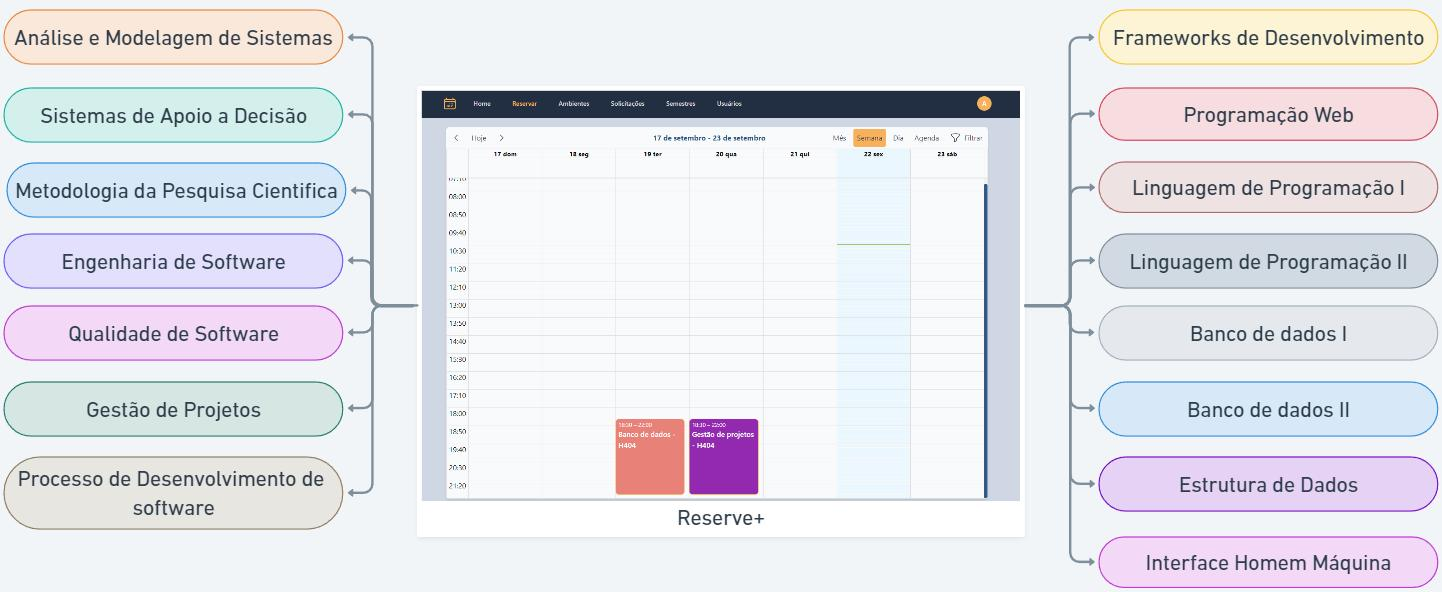
\includegraphics[width=1.0\textwidth]{disciplinas.jpg}
\caption{Disciplinas do Curso de BSI relacionadas à Realização do Reserve+}
\label{fig:disciplinas}
\end{figure}

\end{document}
